{\color{gray}
\section{Software Design Process}
\label{sec:design}
\subsection{Use Cases}
Taken from Ivar Jacobson, see \autoref{fig:usecase20:flow} \cite{jacobson2011usecase}.
\begin{itemize}
	\item popular MoSCoW (Must, Should, Could, Would) prioritization scheme
	\item \gls{use_case} on one card (Priority, Release, Size, Complexity)
	\item \glspl{use_case_slice} generated from use case (Flows, Tests, Estimation)
	\item Find Actors and \glspl{use_case} (slice them subsequently)
	\item Prepare Use Case Slices by describing related stories (use-case narrative) and defining test cases
	\item Analyse Use Case Slices (check how the system elements will interact to perform the use case)
	\item Implement Use Case Slice
	\item Test Use Case Slice
	\item Inspect and Adapt
	\item Test System
\end{itemize}

\subsubsection{Introduction to Use-Cases, Use-Case Flows and Use-Case Slices}

\textbf{\glspl{use_case}} are the general tasks the system and the actors will perform. They are big, not thought completely through and do not contain directly implementable tasks.

\textbf{\glspl{use_case_flow}} are the different flows, how the interaction between actors and the system take place. Usually there is a standard flow, and alternative (error / exception handling) flows. These will be specified later when we go deeper into the analysis. In the state of Use Case Flows we will as well generate Test Cases for the flows. 

\textbf{\glspl{use_case_slice}} are the final development tasks. They will be generated out of the Use Case Flows and can be independently implemented as a single iteration step. They are bases on the Flows and Test Cases. Further Test Cases are usually generated during the implementation react on system specific scenarios.


\begin{figure}[!ht]
\centering
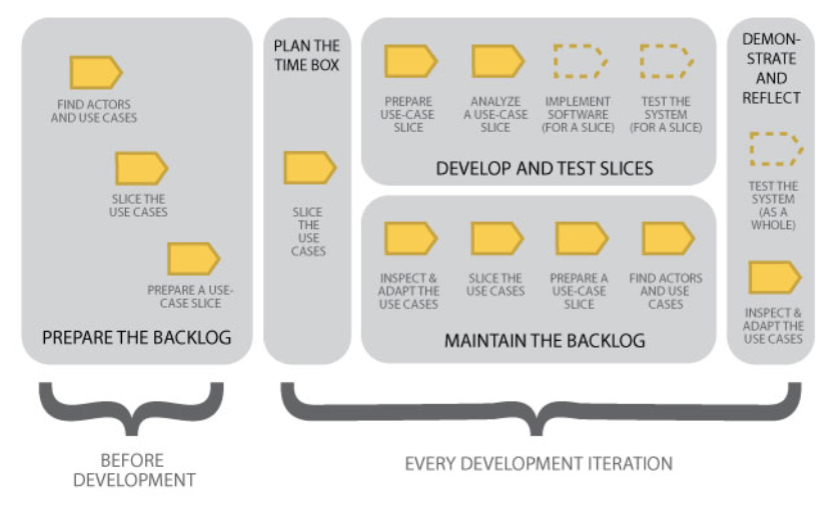
\includegraphics[width=0.8\textwidth]{figures/uc20_flow}
\caption{\gls{use_case} 2.0 activities for iterative development approaches}
\label{fig:usecase20:flow}
\end{figure}


\subsubsection{Actors in this System}
\label{sub:sassoon:actors}
\begin{itemize}
	\item \textbf{Clinician}: main user of the system, does the actual lookup for an applicable model.
	\item \textbf{Statistician}: implements statistical models and defines arguments for them.
	\item \textbf{Data Analyst}: provides data of patients to the system.
	\item \textbf{Academic Researcher}: does in depth analysis of the system and its behaviour.
	\item \textbf{Admin}: Registers new users and has extended rights over data.
\end{itemize}
}

\subsubsection{Use-Cases}

\subsubsection{Use-Case Flows}

\subsubsection{Use-Case Slices}

\subsection{Test Plan}

\subsection{Test Report}


